Using the 4x4 network, we tested the effects of shadowing on the direct transmission path between the source and destination nodes (Figure \ref{fig:4x4topologyshadowing}), as well as between possible diversity nodes, leaving the direct transmission channel unobstructed (Figure \ref{fig:4x4topology}).
We then compared the throughput of direct transmission to our cooperative diversity scheme in both situations.

Figures \ref{fig:4x4throughput} and \ref{fig:4x4throughputshadowing} display the improvement in throughput using the cooperative diversity scheme compared to direct transmission in the scenarios with and without line of sight from the source to the destination, respectively.
The effective throughput displays a significant increase in both scenarios.
In the scenario with significant shadowing in the direct transmission path, the bandwidth utilization is increased from almost 0\% to roughly half of that of the direct transmission with no shadowing.
This is a fair representation of the improvement this scheme could bring to a system where the channel between two communicating nodes contains significant shadowing.
In addition, the maximum likelihood diversity node selection method shows significant throughput gains in both scenarios.  This can be attributed the the non-selection of nodes with poor channels to the destination node due to distance and shadowing.
\begin{figure}
	\centering
	\begin{subfigure}{}
		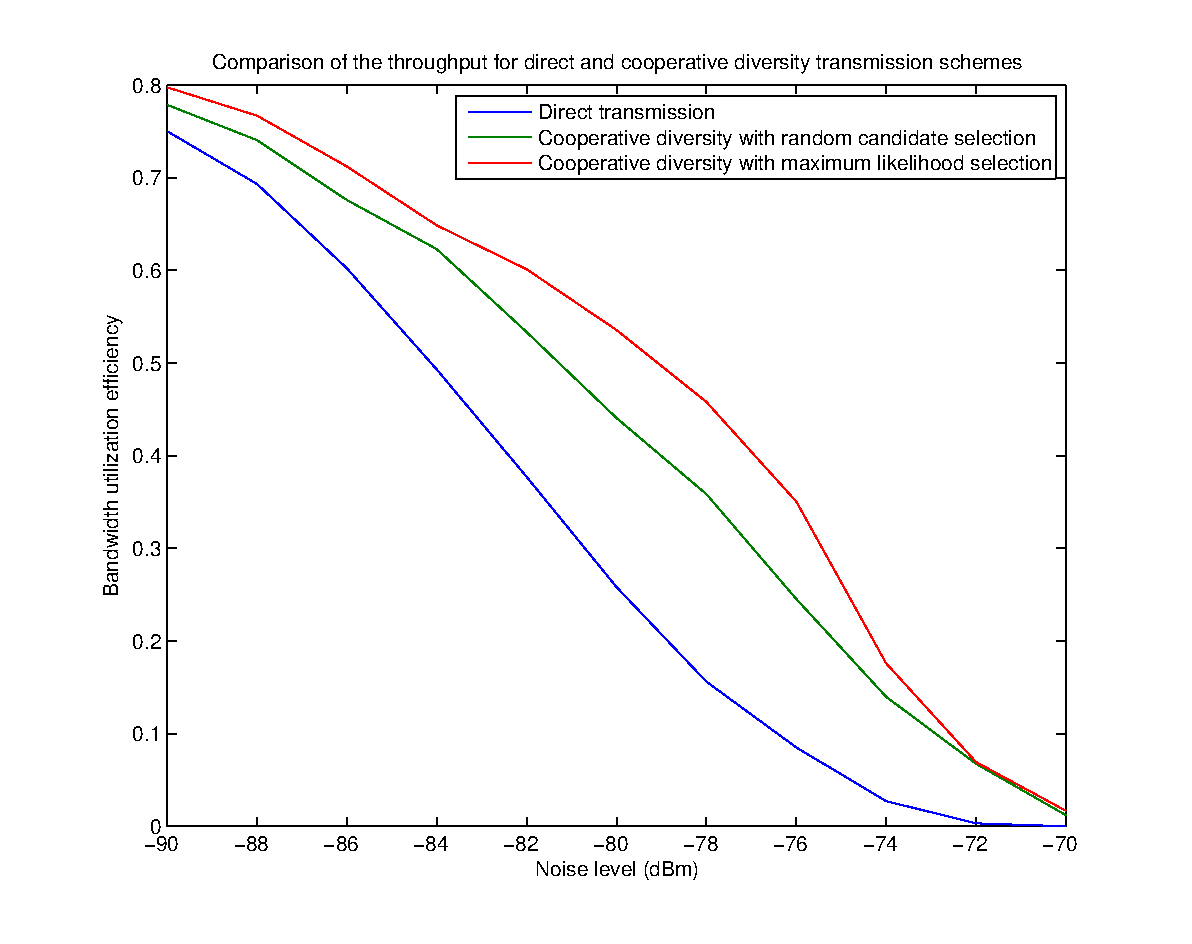
\includegraphics[scale=.45]{figures/4x4throughput}
		\caption{Bandwidth utilization of the 4x4 configuration with line of sight.}
		\label{fig:4x4throughput}
	\end{subfigure}
	
	\vspace{2cm}
	
	\begin{subfigure}{}
		\includegraphics[scale=.4]{figures/4x4throughput_shadowing}
		\caption{Bandwidth utilization of the 4x4 configuration with direct path shadowing.}
		\label{fig:4x4throughputshadowing}
	\end{subfigure}
\end{figure}

In the case of line of sight between the source and destination nodes, cooperative diversity introduces a significant diversity gain in medium to low SNR environments that reduces to an array gain in higher SNR environments.
If nodes expect to have line of sight to other nodes, nodes in the network can disable cooperative diversity in the case of high SNR to decrease the total power consumption of the network without sustaining a significant throughput penalty.
In the case of shadowing in the direct transmission path, this is not the case.
The throughput does not so much depend on the SNR as much as the severe path loss due to the shadowing.
Implementing cooperative diversity in this scenario functions similarly to relaying the data, without the complexity of identifying the source of data loss as poor channel state or shadowing.
In the shadowing example, the benefit of cooperative diversity grows with increasing SNR, but may not be as efficient as a pure relaying scheme.

These simulation results show that cooperative diversity is an effective method of increasing throughput in both shadowing and low SNR environments without the need of identifying the source of data loss.